\documentclass[a4paper, 12pt]{article}
\usepackage[T2A,T1]{fontenc}
\usepackage[utf8]{inputenc}
\usepackage[english, russian]{babel}
\usepackage{graphicx}
\usepackage[hcentering, bindingoffset = 10mm, right = 15 mm, left = 15 mm, top=20mm, bottom = 20 mm]{geometry}
\usepackage{multirow}
\usepackage{lipsum}
\usepackage{amsmath, amstext}
\usepackage{siunitx}
\usepackage{subcaption}
\usepackage{wrapfig}
\usepackage{adjustbox}
\usepackage{enumerate, indentfirst, float}
\usepackage{capt-of, svg}
\usepackage{icomma}

\newenvironment{bottompar}{\par\vspace*{\fill}}{\clearpage}
 
\begin{document}
\begin{titlepage}

\newcommand{\HRule}{\rule{\linewidth}{0.5mm}} % Defines a new command for the horizontal lines, change thickness here

\center % Center everything on the page
 
%----------------------------------------------------------------------------------------
%	HEADING SECTIONS
%----------------------------------------------------------------------------------------

\textsc{\LARGE Московский \\[0.5cm] Физико-Технический Институт}\\[1,5cm] % Name of your university/college
\textsc{\Large Кафедра общей физики}\\[0.5cm] % Major heading such as course name
\textsc{\large Лабораторная работа \textnumero  3.2.6}\\[0.5cm] % Minor heading such as course title

%----------------------------------------------------------------------------------------
%	TITLE SECTION
%----------------------------------------------------------------------------------------

\HRule
\\[0.4cm]
{ \huge \bfseries Исследование гальванометра}
\\[0.2cm] % Title of your document
\HRule
\\[1.5cm]


 
%----------------------------------------------------------------------------------------
%	AUTHOR SECTION
%----------------------------------------------------------------------------------------

%\begin{minipage}{0.4\textwidth}
	\begin{flushleft} \large
		\emph{Студент:}\\
		Павел \textsc{Северилов} \\
		671 группа
	\end{flushleft}
%\end{minipage}

\begin{bottompar}
	\begin{center}
		
\includegraphics[width = 80 mm]{logo.jpg}
	\end{center}
	{\large \today}

\end{bottompar}
\vfill % Fill the rest of the page with whitespace

\end{titlepage}

\section{Цель работы}
Изучение работы высокочувствительного зеркального гальванометра магнитоэлектрической системы в режимах измерения постоянного тока и электрического заряда.

В работе используются: \textit{зеркальный гальванометр с осветителем и шкалой, источник постоянного напряжения, делитель напряжения, магазин сопротивлений, эталонный конденсатор, вольтметр, переключатель, ключи, линейка.}


\subsection*{Теоретическая часть}

\begin{wrapfigure}[15]{l}{5.2cm}
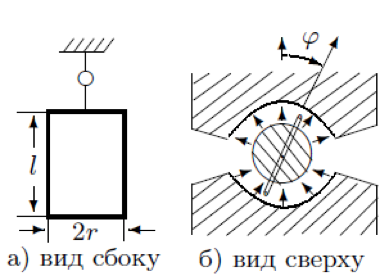
\includegraphics[width=5cm]{t}
\caption{Принцип работы}
\end{wrapfigure} 

		$$\text{Параметры установки:}$$
$$U_0,  = (2.06 \pm 0.02) \text{ В}$$
$$R_2 = 10 \text{ кОм}$$
$$R_0 = 560 \text{ Ом}$$
$$a = (100\pm 1) \text{ см}$$
\vspace{1 cm}

\begin{equation}
J \ddot{\varphi} + \dfrac{\left(BSN\right)^2}{R_{\Sigma}} \dot{\varphi} + D\varphi = BSNI
\end{equation}
$D$ - модуль кручения нити, $\varphi$ - угол поворота рамки от положения равновесия, $B$ - индукция магнитного поля, $N$ - число витков рамки, $I$ - ток в рамке, $S$ - площадь одного витка рамки, $R_{\Sigma}$ - полное сопротивление цепи, $J$ - момент инерции подвижной системы.
Введем обозначения:

\begin{equation}
\left.
\begin{aligned}
&\dfrac{(BSN)^2}{JR_{\Sigma}} = 2\gamma \\
&\dfrac{D}{J} = \omega_0^2 \\
&\dfrac{BSN}{J} = K 
\end{aligned}
\right\}
\end{equation}

Тогда уравнение движения рамки примет вид:
\begin{equation}
\label{eq:diff}
\ddot{\varphi} +2\gamma\dot{\varphi} + \omega_0^2 \varphi = KI
\end{equation}
Величина $\gamma$ называется \textit{коэффициентом затухания} подвижной системы гальванометра,  $\omega_0$ - собственной частотой колебаний рамки.

\subsubsection*{Режим измерения постоянного тока}
При измерении в режиме постоянного тока, когда затухают колебания: $\ddot{\varphi} = \dot{\varphi} = 0$, поэтому угол поворота можно определить формулой:
$$\varphi = \dfrac{KI}{\omega_0^2} = \dfrac{I}{C_I}$$

Постоянная $C_I =I/\varphi= D/NBS$ называется динамической постоянной гальванометра.

\subsubsection*{Свободные колебания рамки}

В отсутствии внешних источников тока ($I = 0$) будем исследовать свободное движение рамки.
Если считать, что $\varphi(0) = 0$, $\dot{\varphi} = \dot{\varphi_0}$, уравнение примет вид:
$$\ddot{\varphi} +2 \gamma \dot{\varphi} + \omega^2_0 \varphi = 0$$

общее решение такого уравнения имеет вид:
\begin{equation}
\varphi = A_1 e^{\lambda_1t} + A_2e^{\lambda_2t}
\label{eq:sol}
\end{equation}


Рассмотрим всевозможные соотношения между $\gamma$ и $\lambda$.

\begin{enumerate}

\item $\gamma < \omega_0$ (колебательный режим)

В таком случае решением уравнения \ref{eq:sol} является 
$$ \varphi = \dfrac{\dot{\varphi}}{\omega}e^{-\gamma t} \sin \omega t,$$
где $\omega^2 = \omega^2_0 - \gamma^2$
В таком режиме мы наблюдаем затухающие колебания с периодом:
$$T = \dfrac{2\pi}{\omega} = \dfrac{2 \pi}{\sqrt{\frac{D}{J} - \frac{(BSN)^4}{(2JR_\Sigma)^2}}}$$

Если $\gamma \ll \omega_0$, то $ \varphi = \dfrac{\dot{\varphi}}{\omega} \sin \omega t,$

\item $\gamma = \omega_0$ (критический режим)

Решение уравнения \ref{eq:sol} в таком случае имеет вид:
$$\varphi = \dot{\varphi	}te^{-\gamma   t}$$
Получаем, что после отклонения система экспоненциально приближается к нулю.

\item $\gamma > \omega_0$ (случай переуспокоенного гальванометра)

Решение в таком случае имеет вид:
$$ \varphi = \dfrac{\dot{\varphi}}{\sqrt{\gamma^2 - \omega_0^2}}e^{-\gamma t} \sh\sqrt{\gamma^2 - \omega_0^2}  t,$$
\end{enumerate}

\subsubsection*{Режим измерения заряда}

Момент инерции рамки искусственно увеличен, поэтому период свободных колебаний будет больше, чем время прохода короткого импульса тока. Будем считать, что рамка не изменяет своего положения при прохождении импульса.

Тогда проинтегрируем \ref{eq:diff}, домножив на $dt$ от $0$ до $\tau$ - время окончания импульса,  и получим:

$$\dot{\varphi} = K q$$
Величина $C_q = q/\varphi_{max}$ называется \textit{баллистической постоянной} гальванометра. Условия, при которых угол отклонения будет максимален при полном отсутствии затухания: $\varphi_\text{max св} = \frac{Kq}{\omega_0}$. 

В критическом режиме: 
$\varphi_\text{max кр} = \frac{Kq}{\omega_0e}$, то есть в $e$ раз меньше, чем в режиме свободных колебаний.

\section{Работа и измерения}


\subsection*{Определение динамической постоянной}

Соберем схему:

	\begin {figure}[H]
		\begin{center}
			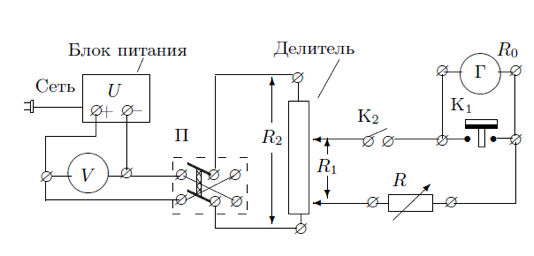
\includegraphics[width = 0.8 \textwidth]{Scheme1}
			\caption{Схема для определения динамической постоянной и критического сопротивления гальванометра}
		\end{center}
	\end {figure}

Угол отклонения рамки будем измерять с помощью осветителя, зеркальца и шкалы, находящейся на расстоянии $a$ от зеркальца. Тогда координата $x$ светового пятна будет выражаться:

$$x=a\tg(2\varphi) \approx 2a\varphi$$
Следовательно динамическая постоянная будет равна 
$$C_I = \dfrac{I}{\varphi} = \dfrac{2aI}{x}$$

Значения силы тока найдем по формуле: $$I = U_0 \dfrac{R_1}{R_2}\dfrac{1}{R+R_0}$$

Запишем полученные значения в таблицу. Также запишем показание $\cfrac{R_1}{R_2}= 1/1000$;

\begin{table}[H]
\centering
\resizebox{\textwidth}{!}{%
\begin{tabular}{|c|c|c|c|c|c|c|c|c|c|c|c|}
\hline
$x, \text{ см}$        & 23.3  & 21.0  & 19.1   & 17.6   & 16.3   & 14.7   & 13.0   & 11.4   & 10.0   & 9.1   & 8.2       \\ \hline
$\sigma_x, \text{ см}$ & 0.1   & 0.1   & 0.1    & 0.1    & 0.1    & 0.1    & 0.1    & 0.1    & 0.1    & 0.1    & 0.1    \\ \hline
$R, \text{ кОм}$        & 18.0 & 20.0 & 22.0 & 24.0 & 26.0 & 29.0 & 33.0 & 38.0 & 43.0 & 48.0 & 53.0  \\ \hline
$I, \text{ нА}$        &110,991&100,195&91,312&83,876&77,560&69,689&61,383&53,423&47,291&42,422 &38,462\\ \hline
$\sigma_I, \text{ нА}$ &1,08&0,97&0,89&0,81&0,75&0,68&0,60&0,52&0,46&0,41&0,37     \\ \hline
\end{tabular}%
}
\caption{Полученные значения}
\end{table}

	\begin {figure}[H]
		\begin{center}
			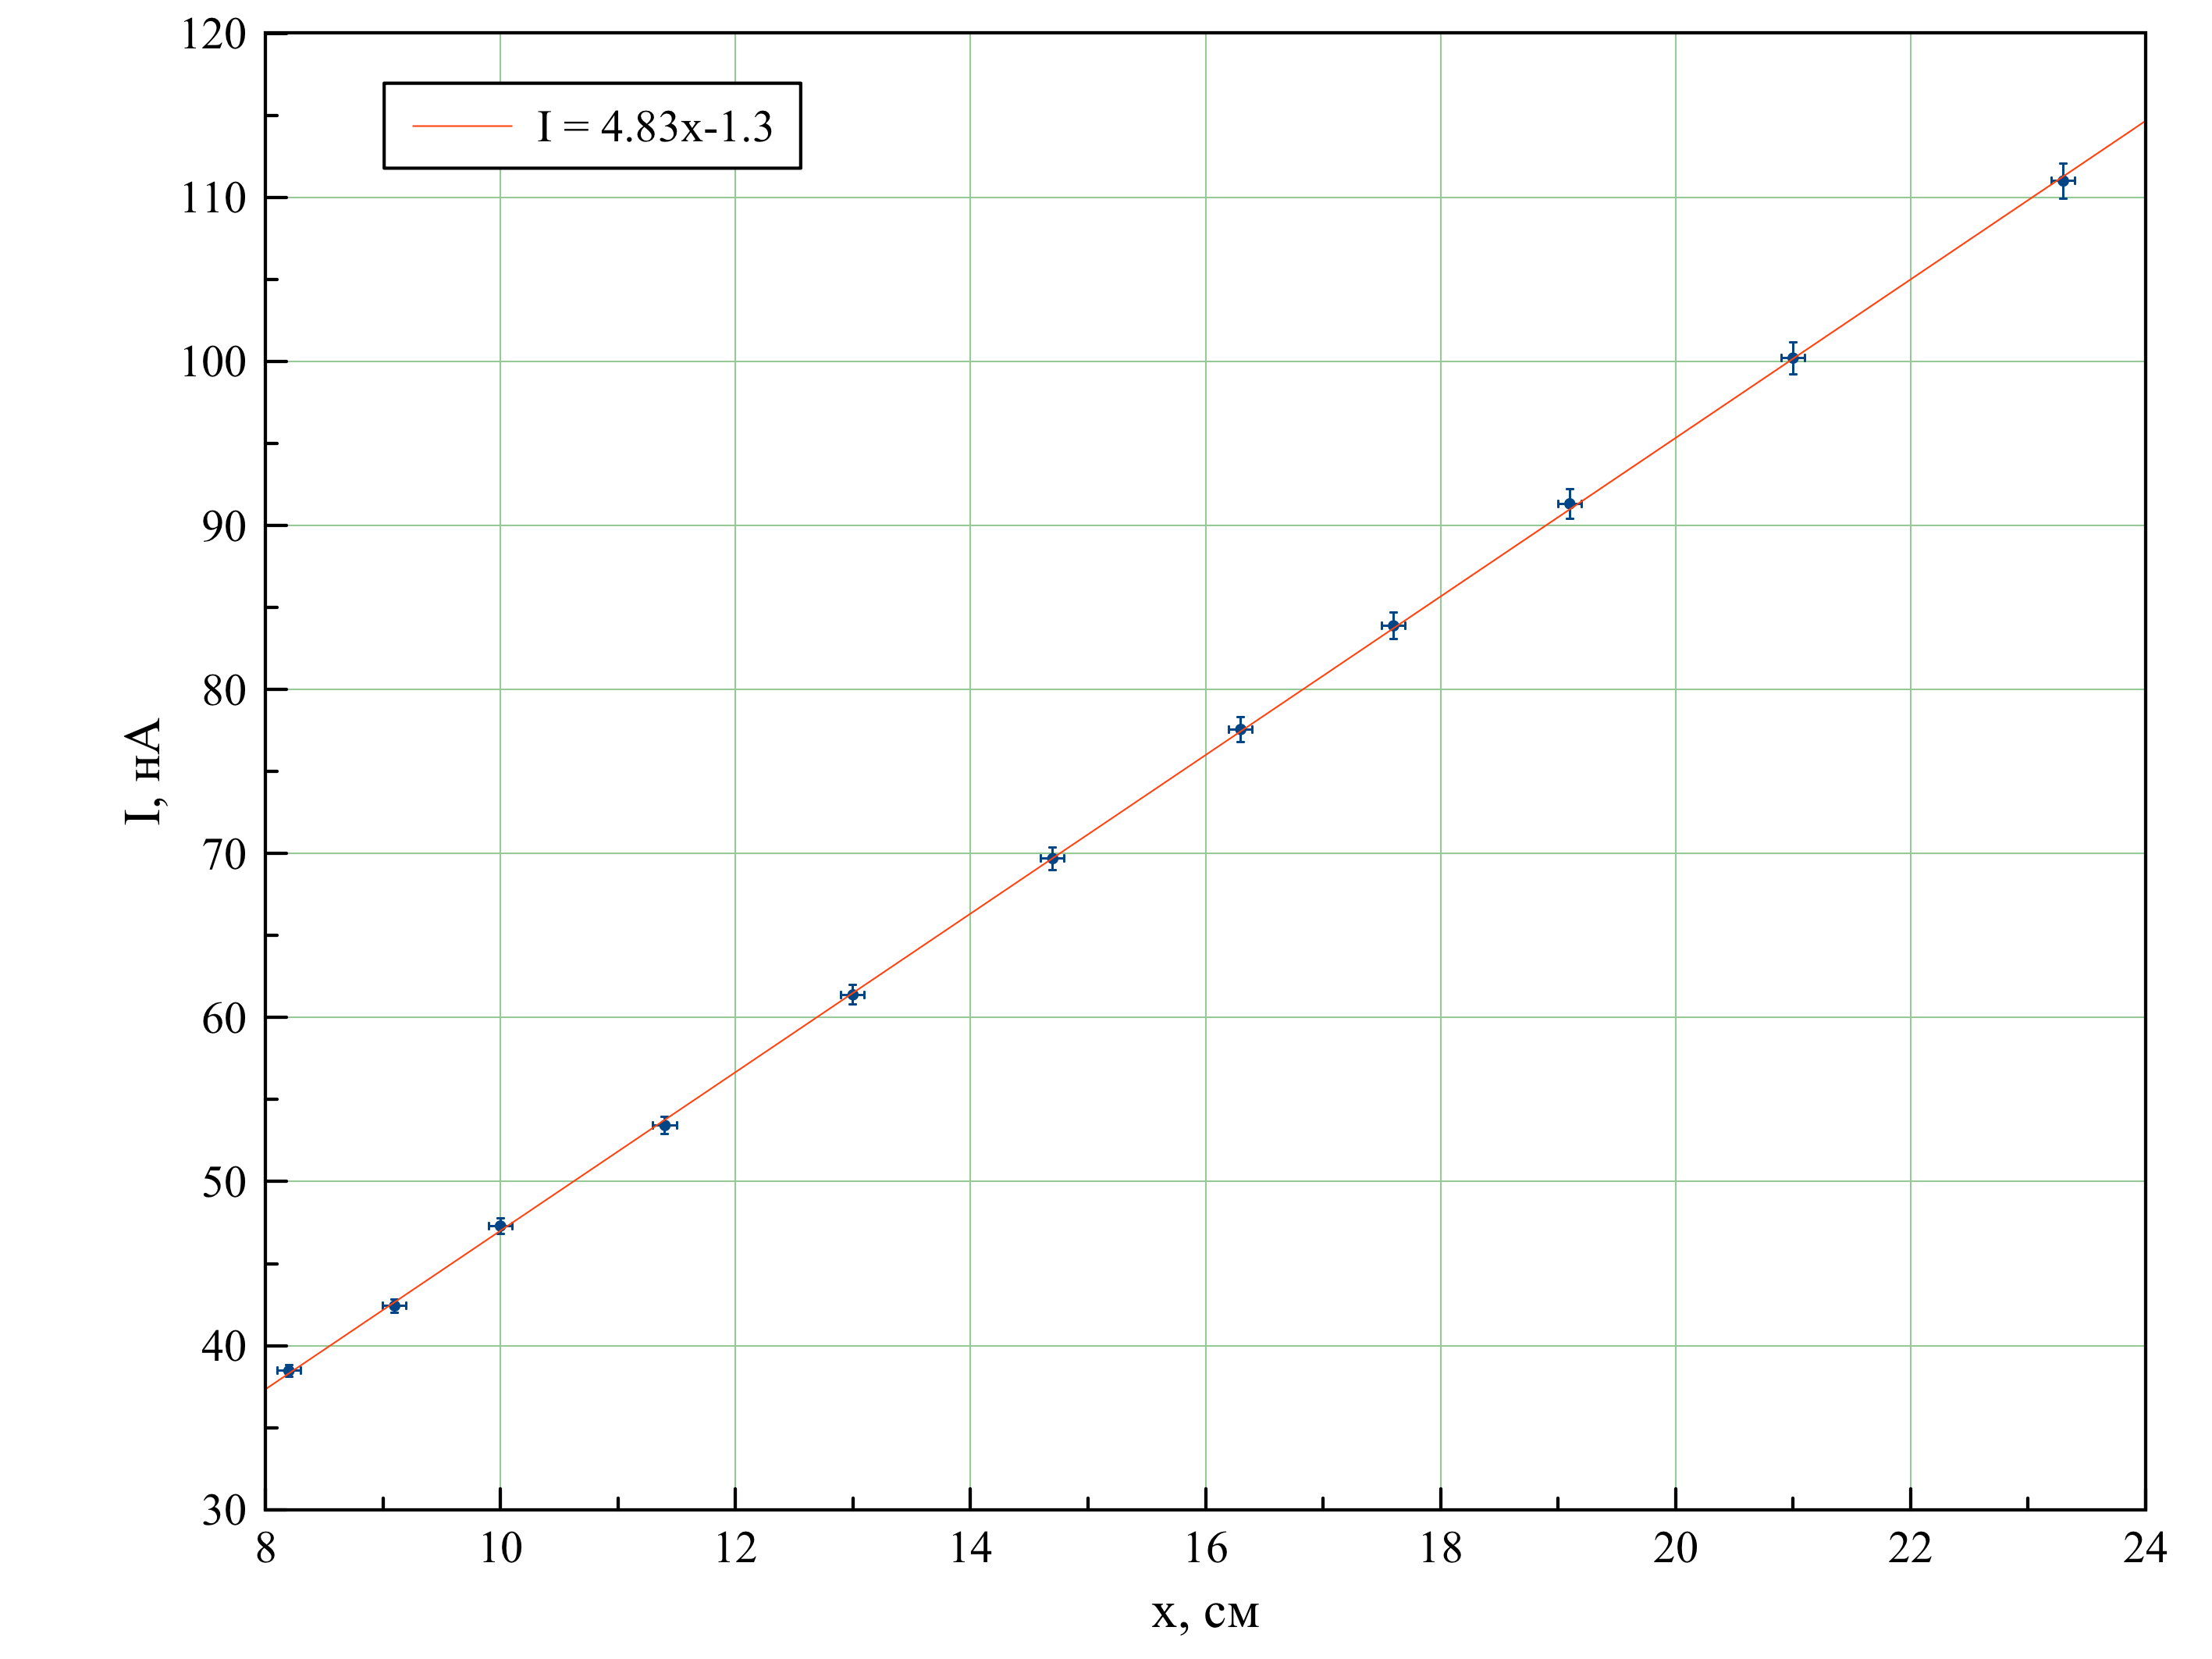
\includegraphics[width = 0.7 \textwidth]{plot1}
			\caption{График зависимости $I = f(x)$}
		\end{center}
	\end {figure}

Из графика получаем значение наклона прямой: $(4,83\pm 0.05)\text{нА/см}$Оно будет равно $\cfrac{I}{x}=\cfrac{C_I}{2a}$. 

Тогда $\boxed{C_I = (9.7 \pm  0.1)10^{-8}\; \dfrac{\text{А $\cdot$ м}}{\text{ мм}}}$
	
\subsection*{Определение критического сопротивления}
Рассчитаем логарифмический декремент затухания $\Theta_0$ размокнутого гальванометра:
$$R = 16.6 \text{ кОм}$$
$$x_n = 19.3 \text{ см}$$
$$x_{n+1} = 15.3 \text{ см}$$
$$\Theta_0 = \ln \dfrac{x_n}{x_{n+1}} = 0.232$$	
Оценим примерное значение периода свободных колебаний:
$$T_0 = 4.9 \text{ с}$$
Оценим значение критического сопротивления, при котором зайчик не переходит за нулевое значение:
$$\boxed{R_{\text{кр}} \approx 8.3 \text{ кОм}}$$
Для рассчета $\Theta$ измерим два последовательных отклонения зайчика в одну сторону. Результаты занесем в таблицу 2.
\begin{table}[H]
\centering
\begin{tabular}{|c|c|c|c|c|c|c|c|}
\hline
$R, \text{ кОм}$ & $x_n$ & $x_{n+1}$ & $\Theta$ &$\sigma_{\Theta}$& $1/\Theta^2$ & $\sigma_{1/\Theta^2}$ & $(R+R_0)^2 \text{ кОм}$ \\ \hline
25&	16,5&	2,0&	2,110&	0,100&	0,225&	0,011&	653,31 \\ \hline
28&	14,7&	2,3&	1,855&	0,087&	0,291&	0,014&	815,67 \\ \hline
31&	13,4&	2,4&	1,720&	0,084&	0,338&	0,016&	996,03 \\ \hline
34&	12,3&	2,6&	1,554&	0,077&	0,414&	0,021&	1194,39 \\ \hline
37&	11,3&	2,7&	1,432&	0,075&	0,488&	0,025&	1410,75 \\ \hline
40&	10,5&	2,8&	1,322&	0,072&	0,572&	0,031&	1645,11 \\ \hline
45&	9,3&	2,8&	1,200&	0,072&	0,694&	0,042&	2075,71 \\ \hline
50&	8,4&	2,8&	1,099&	0,072&	0,829&	0,055&	2556,31 \\ \hline
60&	7,1&	2,8&	0,930&	0,073&	1,155&	0,090&	3667,51 \\ \hline
70&	6,1&	2,7&	0,815&	0,076&	1,505&	0,140&	4978,71 \\ \hline
\end{tabular}
\caption{Исследование зависимости $\Theta$ от $R$}
\end{table}

\begin{equation}
\Theta = \gamma T = 2 \pi \dfrac{\gamma}{\omega} = \dfrac{2 \pi \gamma}{\sqrt{\omega_0^2 - \gamma^2}} = \dfrac{2 \pi R_3}{\sqrt{R_\Sigma^2 - R_3^2}},
\label{eq:critical}
\end{equation}
где введено обозначение:
$$R_3 = \frac{(BSN)^2}{2\sqrt{JD}} = R_0 + R_\text{кр}$$
Тогда при $R = R_\text{кр}$  выполняется: $\Theta \rightarrow \infty$

Получим из \ref{eq:critical} уравнение прямой в координатах $X = (R_0 + R)^2$ и $Y = 1/\Theta^2$:

$$\dfrac{1}{\Theta^2} = \dfrac{(R_0 + R)^2}{4 \pi^2 R_2^3} - \dfrac{1}{4 \pi^2}\Rightarrow R_\text{кр} = \dfrac{1}{2 \pi} \sqrt{\dfrac{\Delta X}{\Delta Y}} - R_0$$


Построим график $\cfrac{1}{\Theta^2}=f((R+R_0)^2)$ по данным из Таблицы 2:
\begin {figure}[H]
	\begin{center}
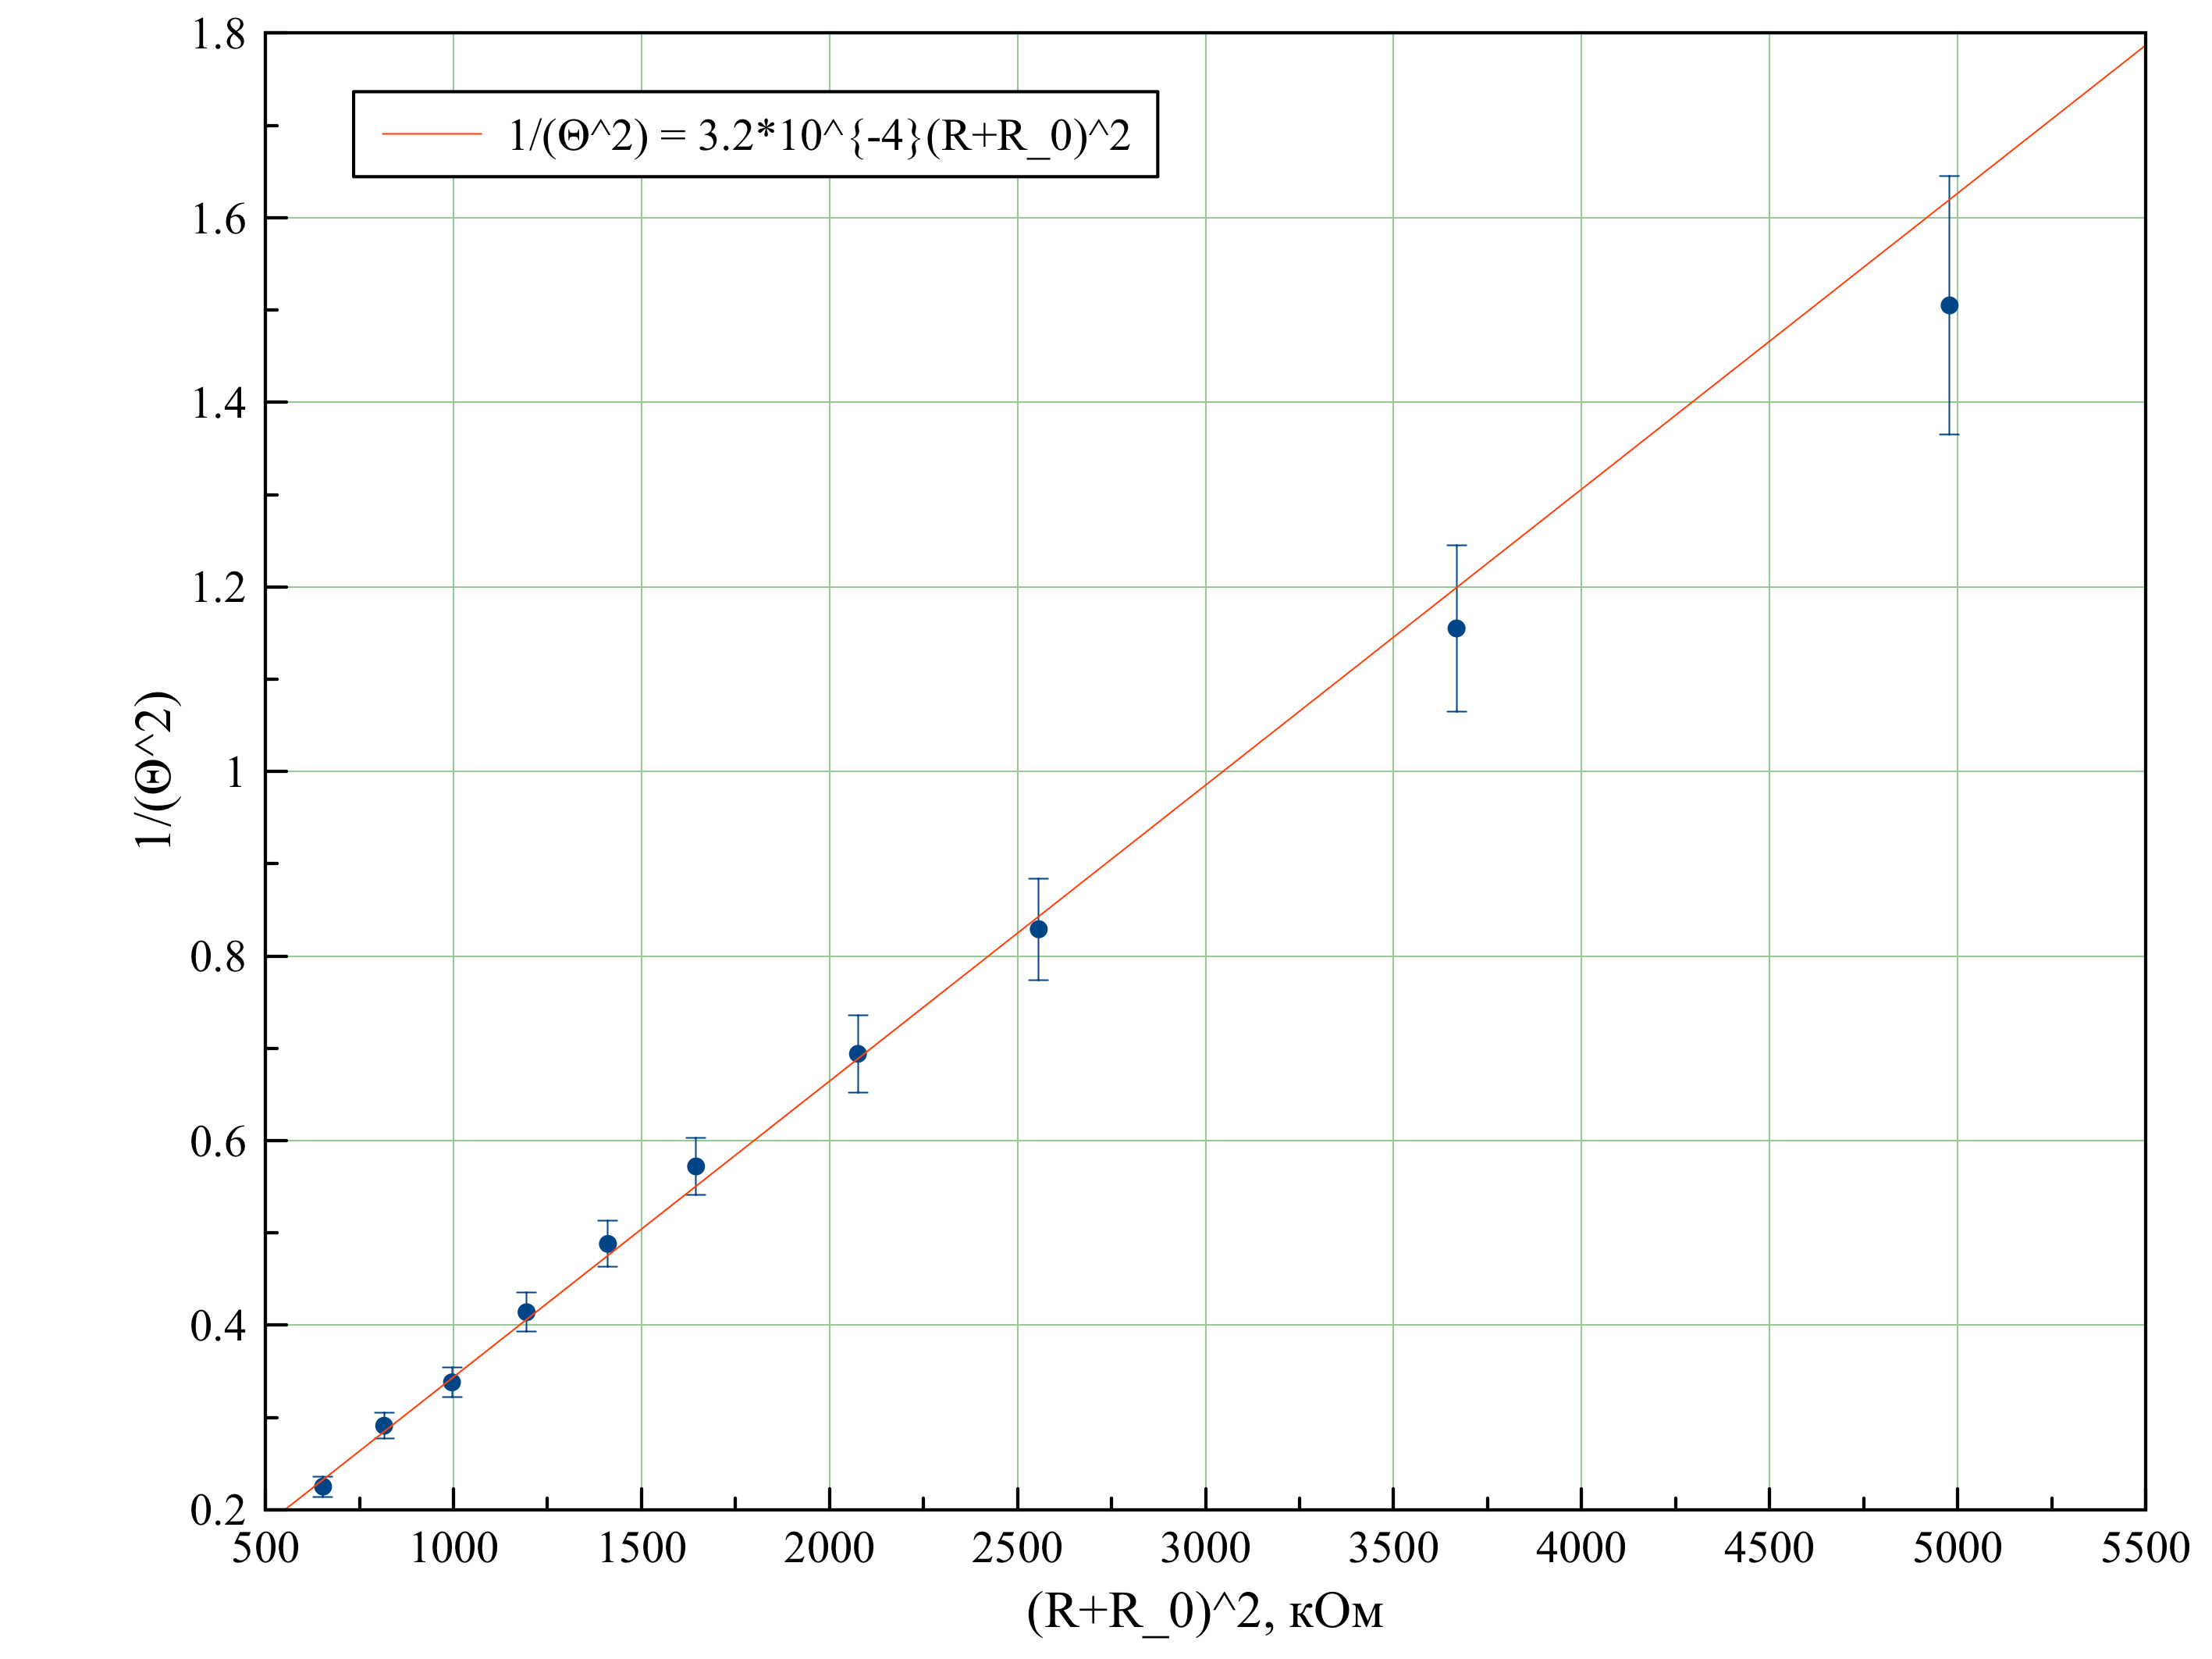
\includegraphics[width = 0.7\textwidth]{plot2}
		\caption{График зависимости $1/\Theta^2 = f((R_0 + R)^2)$}
	\end{center}
\end {figure}


Из графика $\dfrac{\Delta Y}{\Delta X} = (3.2 \pm 0.32)\cdot10^{-4}\text{ кОм}^{-2}$, поэтому 
$$\boxed{R_\text{кр} = (8.34 \pm 0.77) \text{  кОм}}$$

\subsection*{Баллистический режим}

$$C = 2 \text{ мкФ}$$
$$R_1/R_2 = 1/40$$
$$l_{max} = 23.5 \text{ см}$$
$$\sigma_{l_{max}}=0.2 \text{ см}$$
Соберем схему:

\begin {figure}[H]
	\begin{center}
		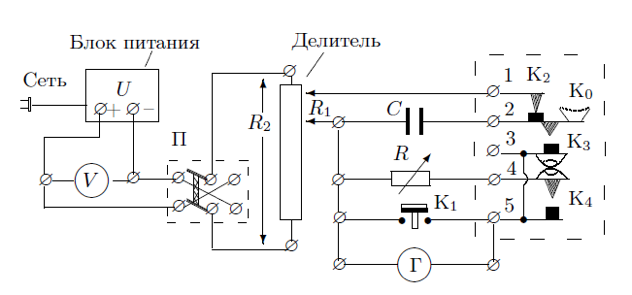
\includegraphics[width = 0.8 \textwidth]{Scheme2}
		\caption{Схема для определения баллистической постоянной и критического сопротивления гальванометра, работающего в баллистическом режиме}
	\end{center}
\end {figure}

\begin{table}[H]
\centering
\begin{tabular}{|c|c|c|}
\hline
$R, \text{ Ом}$ & $l_{max}$ &  $(R+R_0)^{-1}, \; \text{кОм}^{-1}$ \\ \hline
 50	&19,6	& 0,0198 \\ \hline
 45	&19,4	& 0,0219 \\ \hline
40	&19,0	& 0,0247 \\ \hline
35	&18,5	& 0,0281 \\ \hline
30	&17,9	&0,0327 \\ \hline
25	&17,5	&0,0391 \\ \hline
20	&16,4	&0,0486 \\ \hline
15	&14,6	&0,0643 \\ \hline
10	&12,8	&0,0947 \\ \hline
5	&9,5	&0,1799          \\ \hline
\end{tabular}
\caption{Исследуем зависимость между $l_{max}$ и $R$}
\end{table}

\begin {figure}[H]
	\begin{center}
		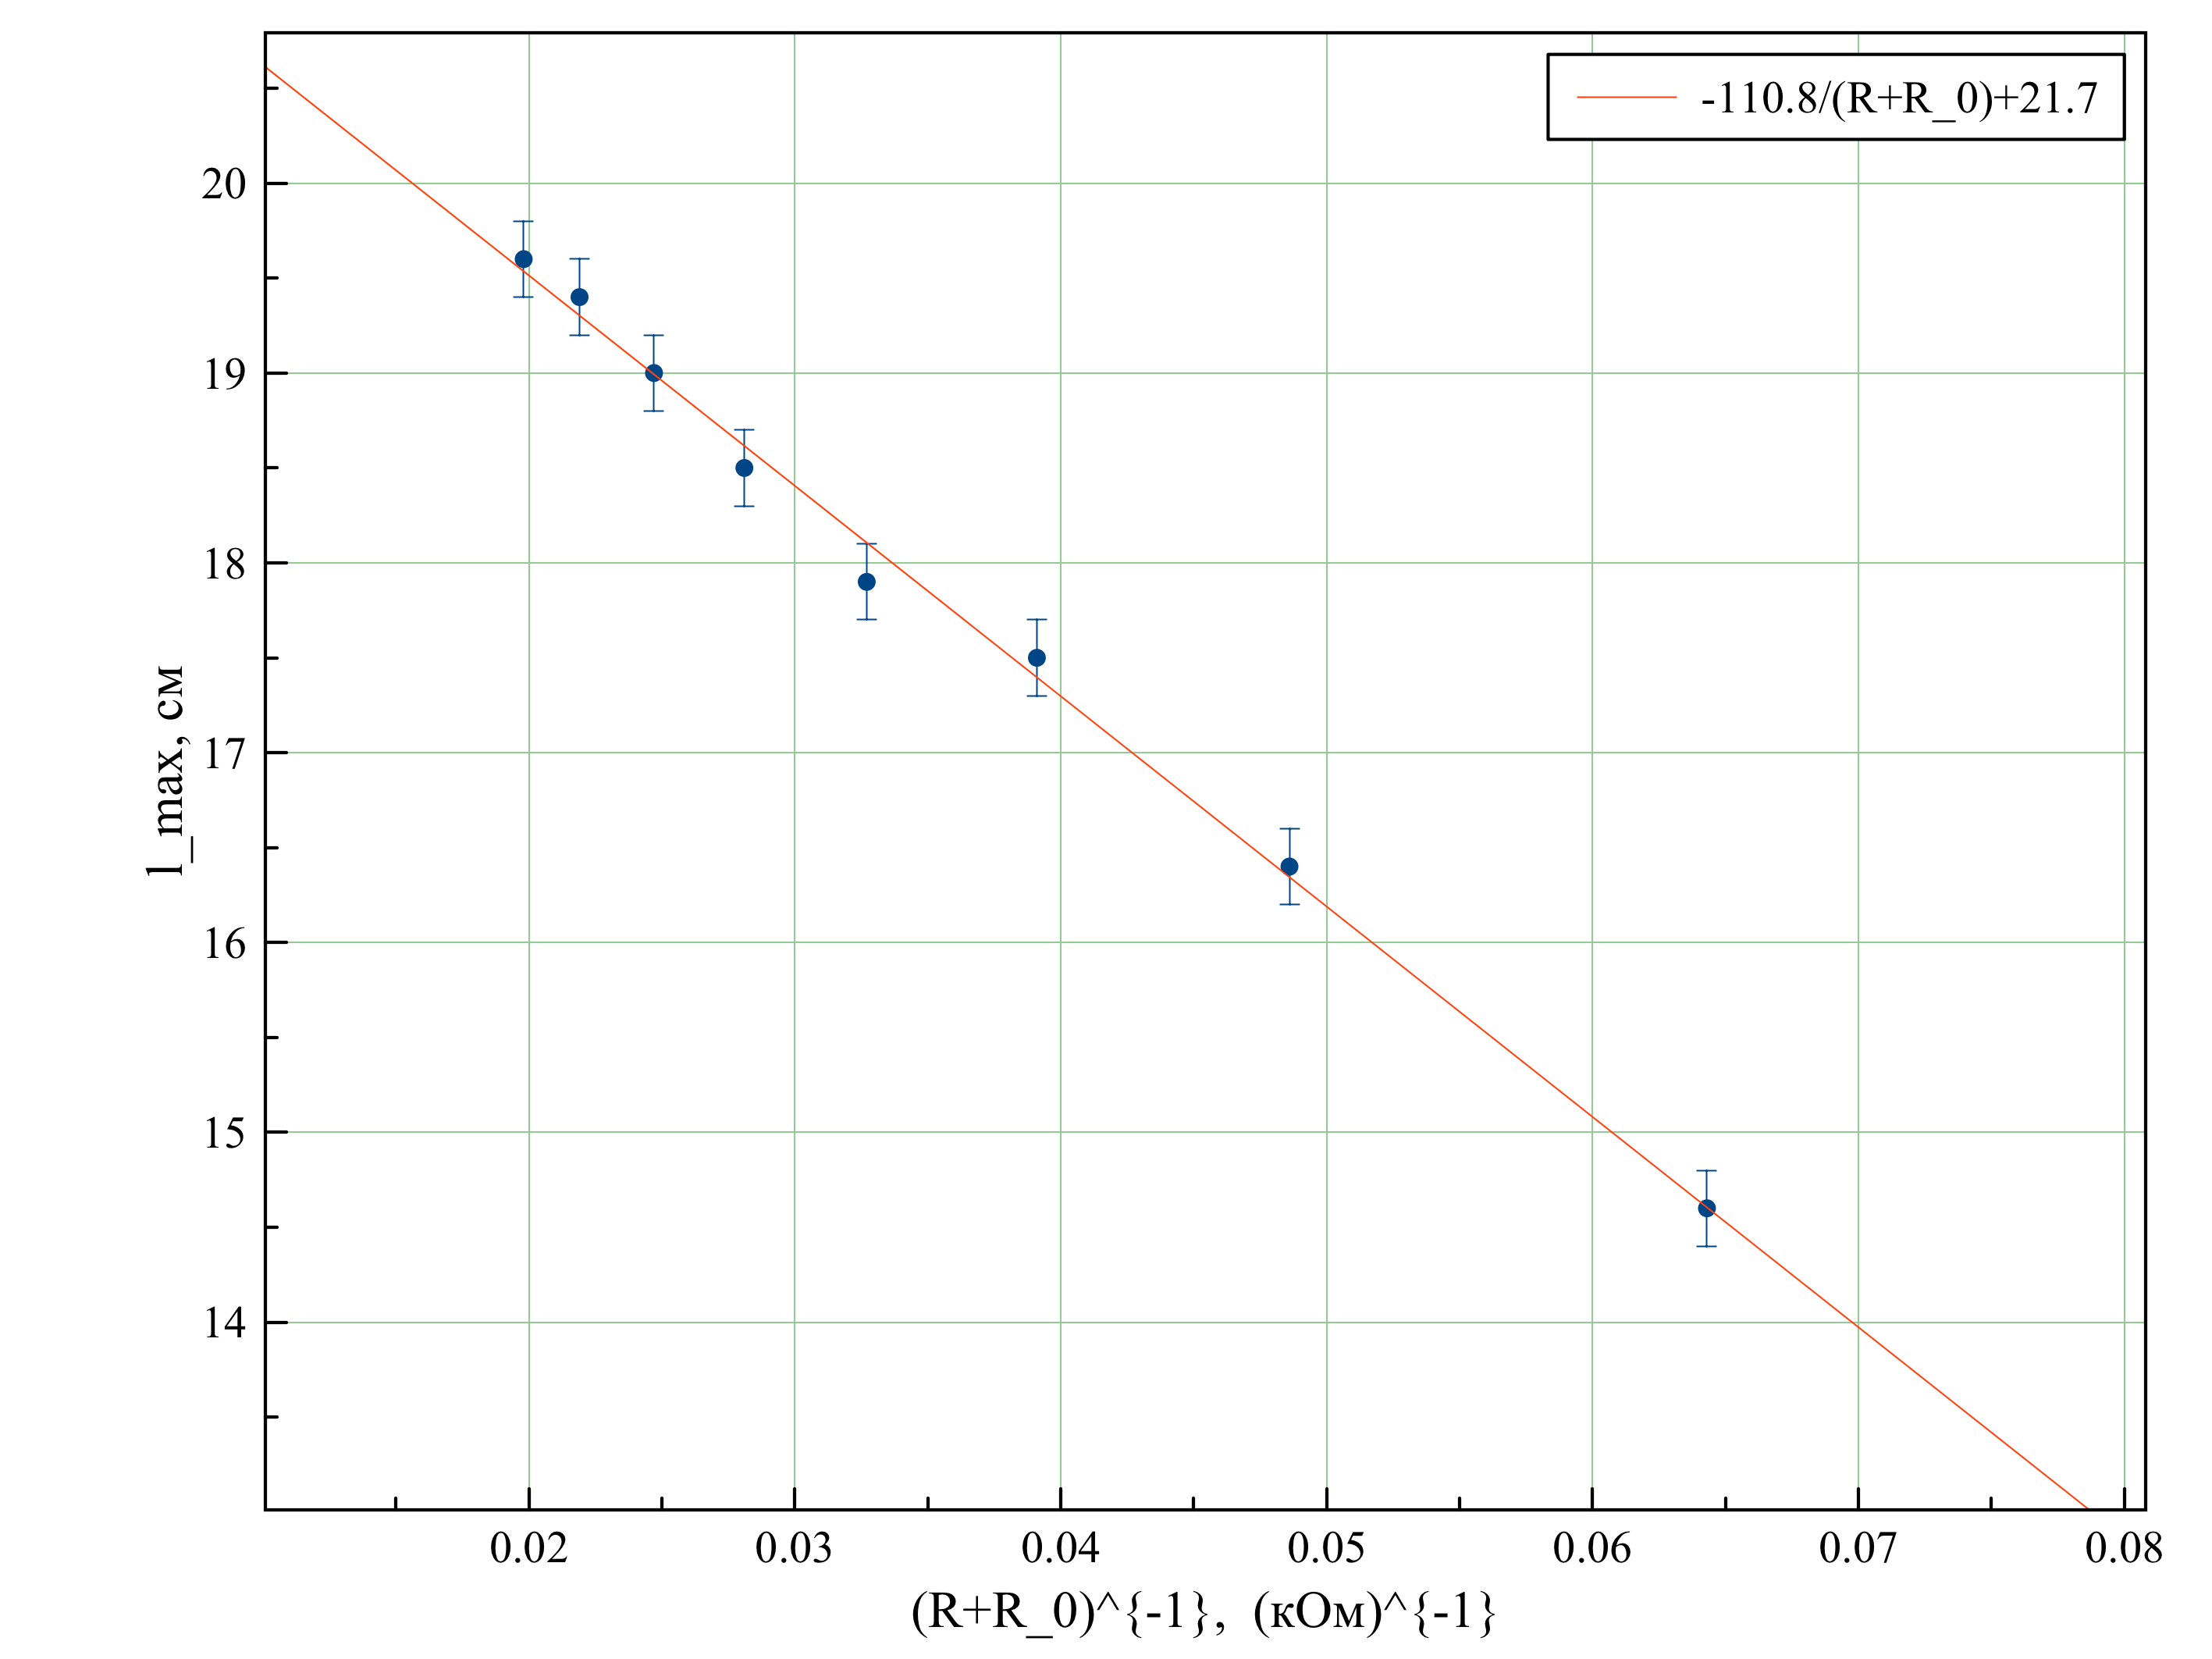
\includegraphics[width = 0.8 \textwidth]{plot3}
		\caption{Зависимость $l_{max} = f[(R_0+R)^{-1}]$}
	\end{center}
\end {figure}

Определим значение $R_\text{кр}$ по графику: значение максимального отклонения в критическом режиме в $e$ раз меньше, чем в режиме свободных колебаний. Зная зависимость $l_{max} = f[(R_0+R)^{-1}]$ найдем значение критического сопротивления
$$l =\cfrac{-110.8}{R+R_0}+21.4;~~~~~~l\equiv\cfrac{l_{max}}{e}$$
$$\Rightarrow \boxed{R_{\text{ кр}} = \cfrac{110.8}{21.4-\cfrac{l_{max}}{e}}-0.56 = (8.13\pm 0.65) \text{ кОм}}$$

Определим баллистическую постоянную гальванометра $C_{Q_\text{кр}} \left[\dfrac{\text{К}}{\text{мм/м}} \right]$:

$$C_{Q_\text{кр}} = \dfrac{q}{\varphi_{max \text{ кр}}} = 2a \dfrac{R_1}{R_2} \dfrac{U_0C}{l_{max \text{ кр}}} = 8.77\cdot 10^{-10} \cfrac{\text{м}\cdot\text{К}}{\text{мм}}$$

Время релаксации $t = R_0C = 560 \cdot 2 \cdot 10^{-6} = 1.12 \cdot 10^{-3} \text{ с} \ll T_0 = 4.9 \text{ с}$

\section{Вывод}

В данной работе мы измерили значение динамической постоянной гальванометра, критического сопротивления тремя способами и баллистической постоянной. Получили, что все три $R_\text{кр}$: вычисленное подбором, по графику стационарного режима и по графику баллистического режима -- совпадают с учетом погрешностей. Наибольшая ошибка в третьем эксперименте, так как большой вклад в погрешность дает скорость реакции человека -- отклонения зайчика происходят быстро, необходимо успевать замыкать ключ и считывать значения.

\end{document}